\section{Reimplementation Results} \label{sec:reimplementation-results}

Figure \ref{fig:original_plot} shows the results from the original paper and Figure \ref{fig:combined_plot} shows the reimplementation results.
It can be seen that both plots show the same trajectory for the fitness over the series of function evaluations.
The reimplementation plots show slightly rougher due to the lower number of experiments used to calculate the average performance. 

\begin{figure}[ht!]
    \centering 
    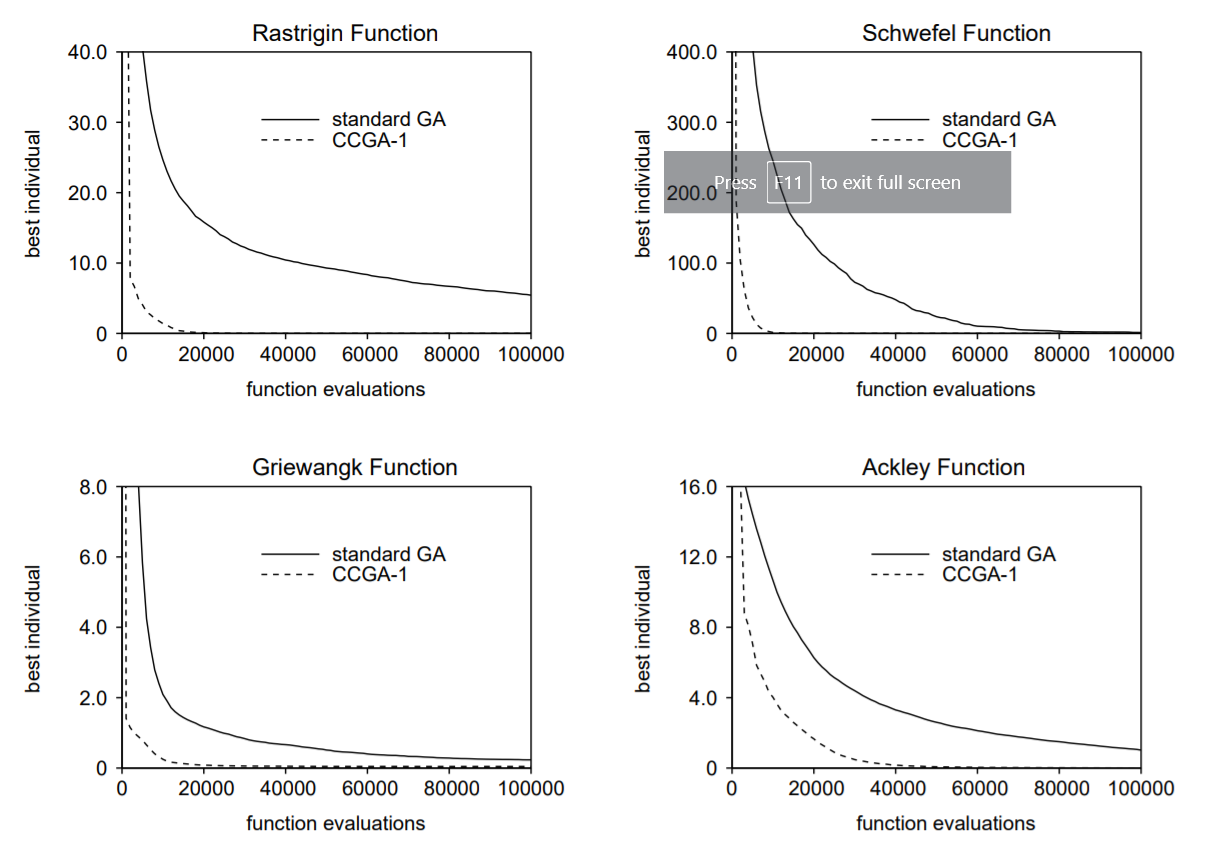
\includegraphics[width=0.9\textwidth]{img/original_plot.png}
    \caption{The figure this assignment aims to reimplement. Reproduced from\cite{original-paper}.}
    \label{fig:original_plot}
  \end{figure}

  \begin{figure}[ht!]
    \centering 
    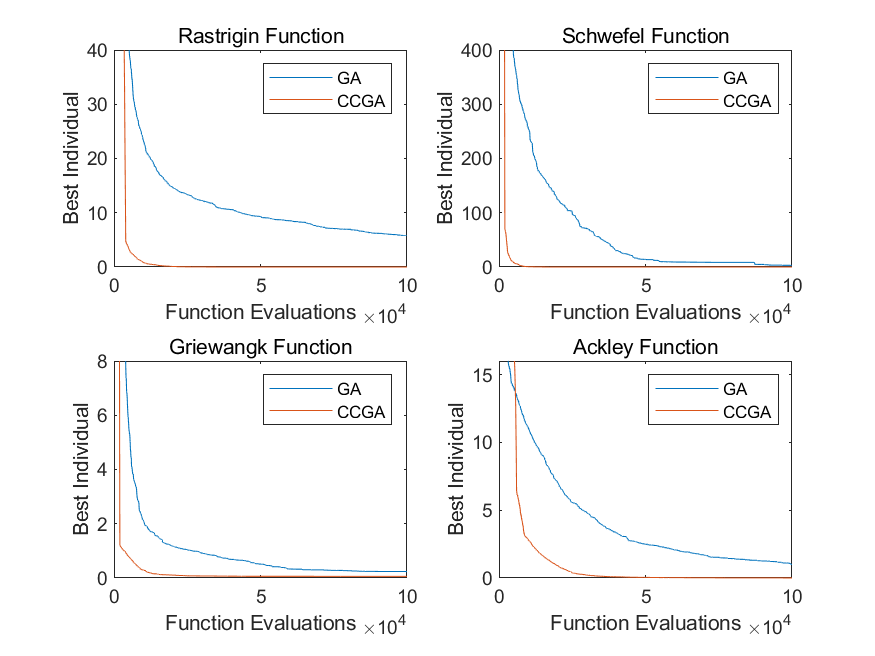
\includegraphics[width=0.9\textwidth]{img/combined_plot.png}
    \caption{The figure produced by this reimplementation.}
    \label{fig:combined_plot}
  \end{figure}
